\documentclass{article}

\usepackage{graphicx}
\usepackage{tikz}
\usepackage{tikzsymbols}
\usetikzlibrary{calc,patterns,shapes.geometric}
\pagestyle{empty}
\usepackage[margin=0pt]{geometry}
\geometry{papersize={14in,12in}}

\def\centerarc[#1](#2)(#3:#4:#5){\draw[#1] ($(#2)+({#5*cos(#3)},{#5*sin(#3)})$) arc (#3:#4:#5);}

\begin{document}
	\begin{figure}
		\centering
		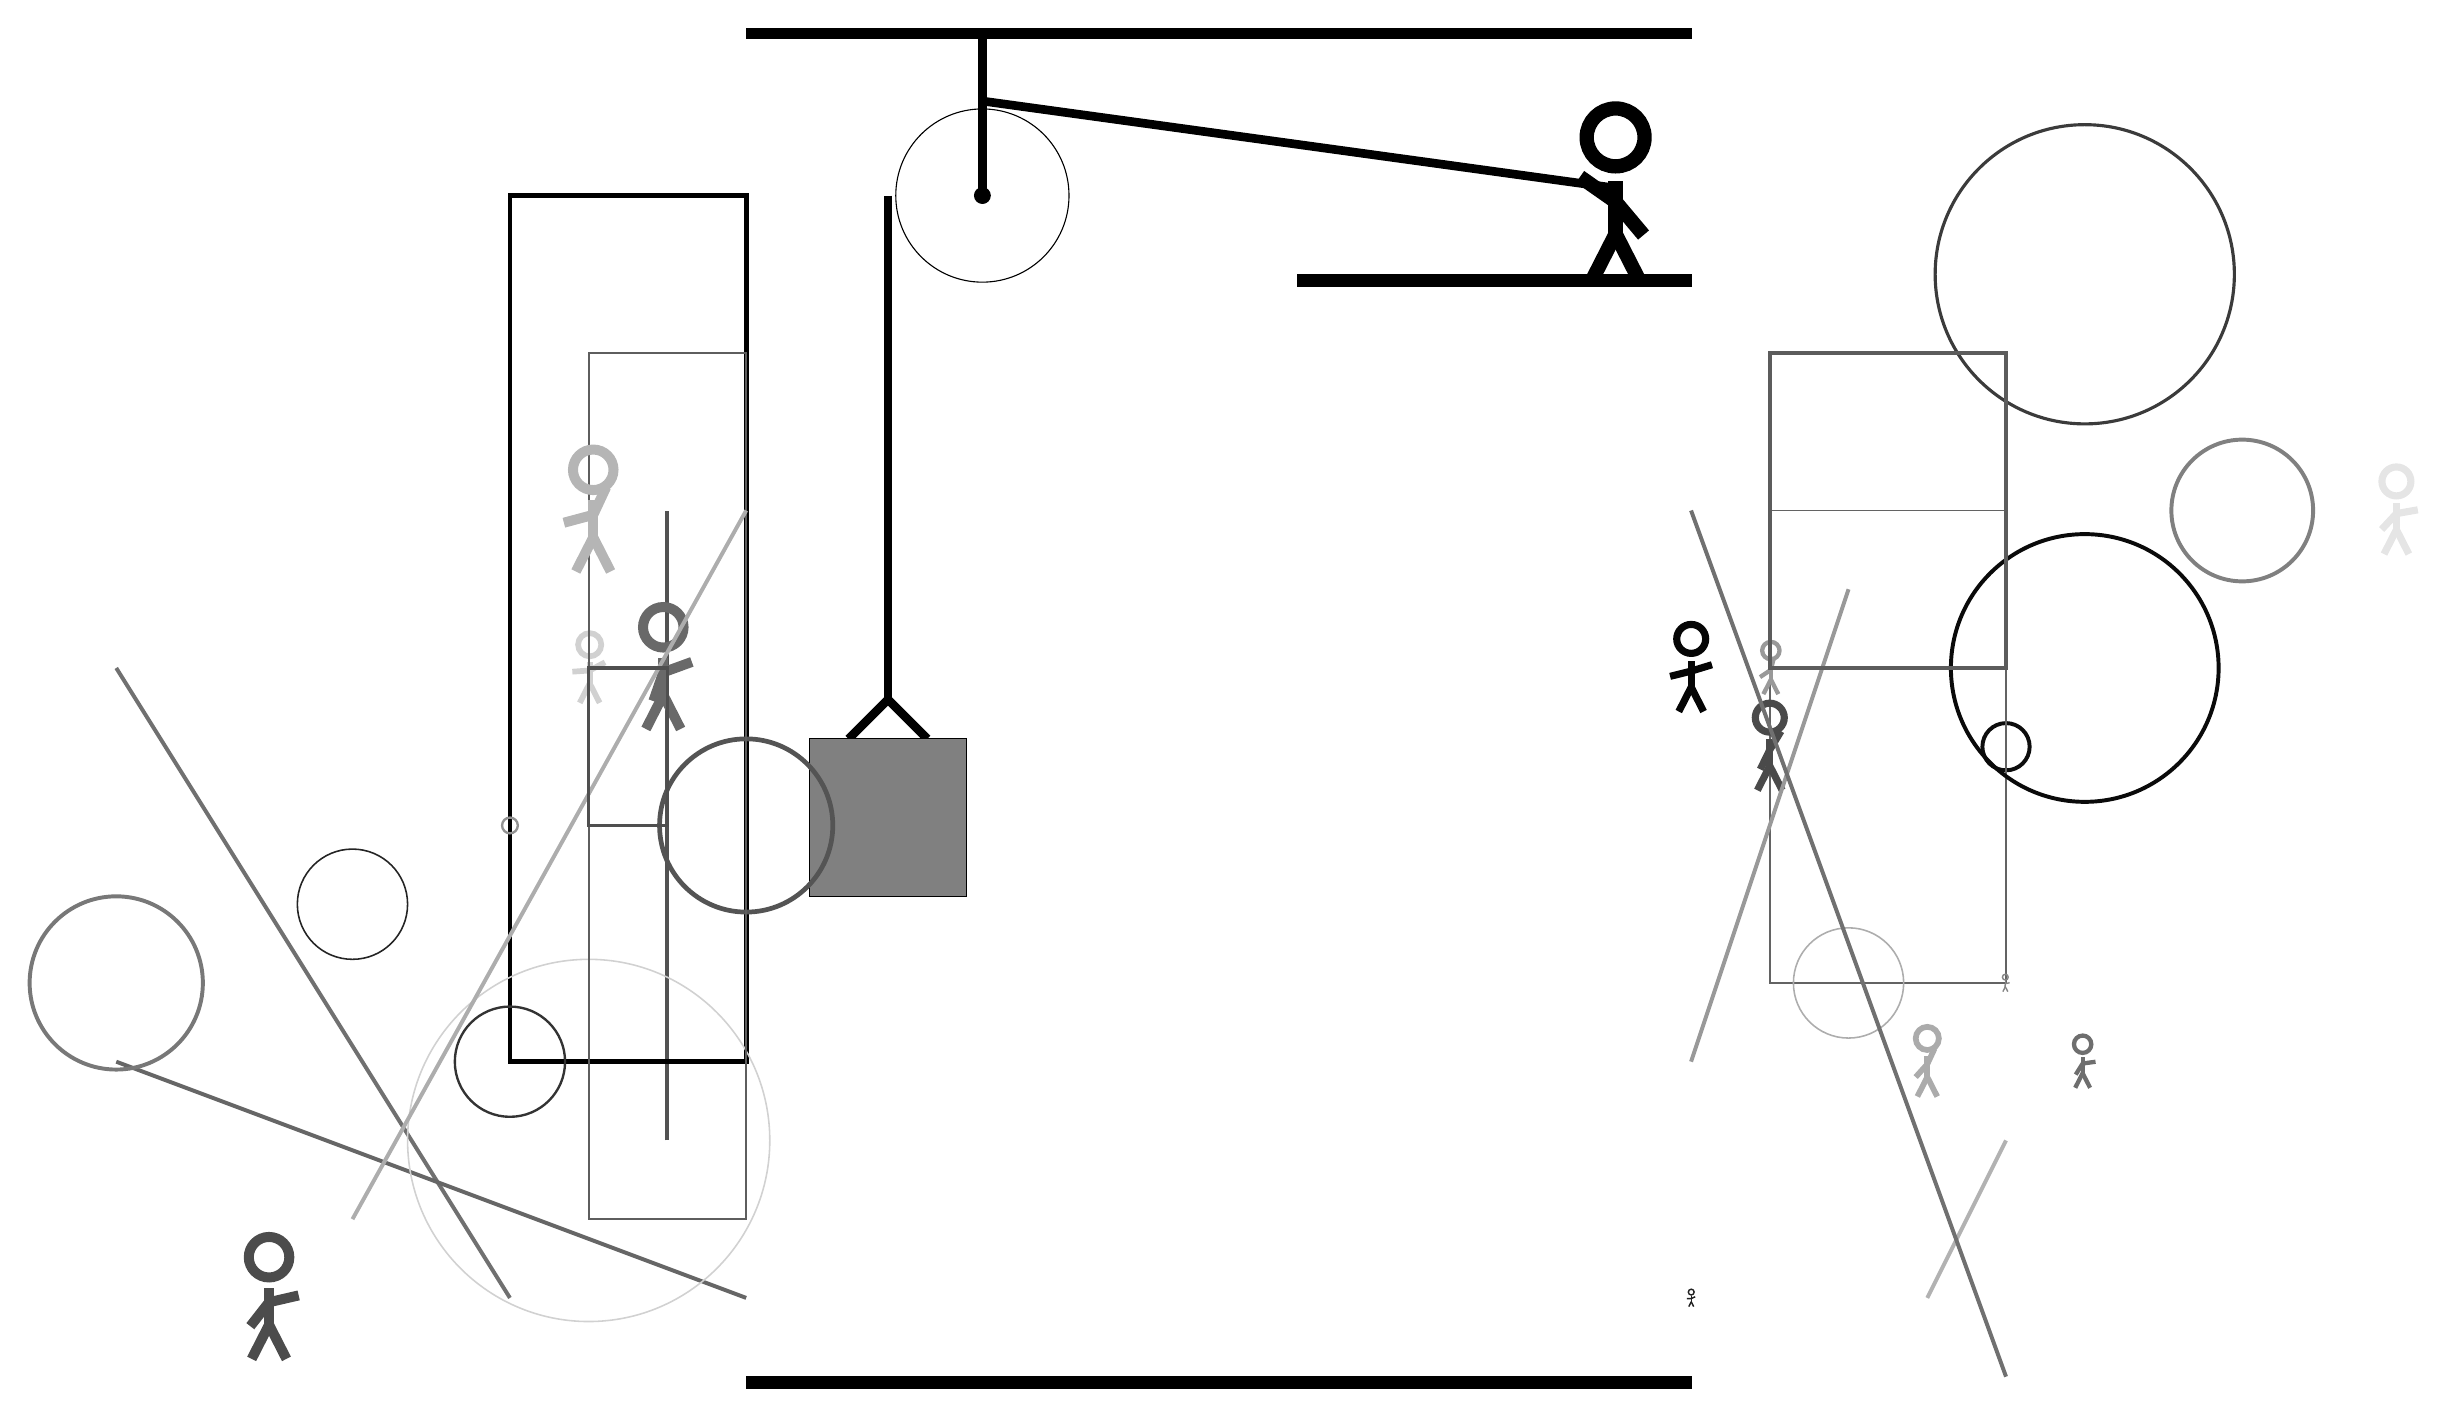
\begin{tikzpicture}
			%%%%% START %%%%%
			
			\draw[fill=black] (-2, 14) rectangle (10, 14.125);
			
			\draw (1, 12) circle (1.1);
			\draw[fill=black] (1, 12) circle (0.1);
			\draw[line width=1.1mm] (1, 14) -- (1, 12);
			
			\draw[line width=1.1mm](-0.7, 5.1) --  (-0.2, 5.6) -- (0.3, 5.1);
			\draw[fill=black!50] (-1.2, 5.1) rectangle (0.8, 3.1);
			
			\draw[line width=1.1mm](-0.2, 12) -- (-0.2, 5.6);
			\centerarc[line width=1.1mm](1, 12)(90:180:1.2000000000000002)
			\draw[line width=1.1mm](1, 13.2) -- (9, 12.1);
			
			\draw[line width=0.5mm, color=black!30](14, 0) -- (13, -2);
			
			\draw [line width=0.2mm, color=black!86](-7, 3) circle (0.7);
			\draw[line width=0.5mm, color=black!68](-3, 0) -- (-3, 8);
			\node[line width=0.6mm, color=black!18] at (-4, 6) {\Strichmaxerl[4][4][28]};
			
			\draw[line width=0.6mm, color=black!100] (-2, 12) rectangle (-5, 1);
			\draw [line width=0.5mm, color=black!95](14, 5) circle (0.3);
			\node[line width=0.6mm, color=black!87] at (10, -2) {\Strichmaxerl[1][2][24]};
			
			\draw[line width=0.2mm, color=black!61] (11, 2) rectangle (14, 8);
			\node[line width=0.5mm, color=black!48] at (14, 2) {\Strichmaxerl[1][85][10]};
			
			\draw[line width=0.5mm, color=black!56](-5, -2) -- (-10, 6);
			\draw [line width=0.6mm, color=black!67](-2, 4) circle (1.1);
			\node[line width=0.2mm, color=black!98] at (10, 6) {\Strichmaxerl[5][14][17]};
			\draw[line width=0.5mm, color=black!60](-2, -2) -- (-10, 1);
			
			\node[line width=0.4mm, color=black!71] at (11, 5) {\Strichmaxerl[5][64][59]};
			\draw [line width=0.5mm, color=black!96](15, 6) circle (1.7);
			\node[line width=0.3mm, color=black!10] at (19, 8) {\Strichmaxerl[5][47][10]};
			\draw [line width=0.2mm, color=black!18](-4, 0) circle (2.3);
			\node[line width=0.6mm, color=black!40] at (11, 6) {\Strichmaxerl[3][34][76]};
			\draw[line width=0.3mm, color=black!63] (-2, 10) rectangle (-4, -1);
			\draw [line width=0.3mm, color=black!80](-5, 1) circle (0.7);
			\node[line width=0.6mm, color=black!59] at (-3, 6) {\Strichmaxerl[7][71][20]};
			\draw [line width=0.4mm, color=black!74](17, 8) circle (0.0);
			
			\draw [line width=0.5mm, color=black!50](17, 8) circle (0.9);
			\draw[line width=0.5mm, color=black!32](-7, -1) -- (-2, 8);
			\draw [line width=0.2mm, color=black!32](12, 2) circle (0.7);
			\draw[line width=0.5mm, color=black!14] (11, 0) rectangle (11, 0);
			
			\draw [line width=0.4mm, color=black!77](15, 11) circle (1.9);
			\draw [line width=0.5mm, color=black!53](-10, 2) circle (1.1);
			\node[line width=0.5mm, color=black!70] at (-8, -2) {\Strichmaxerl[7][52][13]};
			
			\draw[line width=0.5mm, color=black!40](12, 7) -- (10, 1);
			\draw[line width=0.4mm, color=black!69] (-3, 4) rectangle (-4, 6);
			\node[line width=0.6mm, color=black!57] at (15, 1) {\Strichmaxerl[3][58][8]};
			\draw[line width=0.5mm, color=black!64] (11, 10) rectangle (14, 6);
			
			\node[line width=0.4mm, color=black!33] at (13, 1) {\Strichmaxerl[4][48][65]};
			
			\draw[line width=0.5mm, color=black!56](10, 8) -- (14, -3);
			\node[line width=0.3mm, color=black!29] at (-4, 8) {\Strichmaxerl[7][15][65]};
			\draw [line width=0.3mm, color=black!43](-5, 4) circle (0.1);
			
			
			\node at (9, 12) {\Strichmaxerl[10][-35][-50]};
			\draw[fill=black] (5, 11) rectangle (10, 10.85);
			
			\draw[fill=black] (-2, -3) rectangle (10, -3.15);
			
			%%%%% END %%%%%
		\end{tikzpicture}
	\end{figure}	
\end{document}